\label{sec:6}

%%%%%%%%%%%%%%%%%%%%%%%%%%%%% 
% (FURIC) Production Testing
%%%%%%%%%%%%%%%%%%%%%%%%%%%%%

A Production Test Site is currently being assembled at the Univeristy of Florida to perform QC of all the packaged ColdADC ASIC.  The production QC procedure was developed and tested on the first 33 packaged chips at BNL. In this section, we describe the production test system and the results from the first 33 chips.

\subsection{Test Setup}
\label{sec:6.1}
The ColdADC QC teststand is a dedicated system to characterize the ColdADC performance with a low distortion 
signal generator SRS DS360, which is very similar to the test setup described in Section~\ref{sec:2.2}.  
Shown in Figure~\ref{fig:prodQC_blockdiagram} is the block diagram of the setup. The testboard has an ASIC 
socket mezzanine card to avoid having to solder the ColdADC chips. 
This convenience, however, introduces additional capacitance from the ASIC socket which may slightly degrade the test results.
Since the main purpose of the production testing is to distinguish good chips from bad chips, the performance degradation 
from the additional capacitance is not an issue. 
Instead of an on-board oscillator to provide 100MHz clock for FPGA Mezzanine, an external clock source SRS CG635 is used to provide a 
stable clock for both room temperature and liquid nitrogen operations. For ENOB/FFT measurements, clock synchronization between the 
board and the signal generator is required.  Without an external clock source it can be difficult to obtain a stable synchronization 
between the testboard and the signal generator. 
%In fact, for internal ADC core measurements (8 MHz Nyquist bandwidth), 
%unwanted spikes at 2 MHz and 6 MHz can appear at cold. This issue is strongly mitigated by adding an external clean clock source. 
%So, the teststand is updated with the CG635 generator sends a 100 MHz clock to the board and a 10 MHz synchronized signal to the DS360. 
Figure~\ref{fig:prod_warmsetup} shows the test setup at room temperature.
\begin{figure}[h!]
\centering
  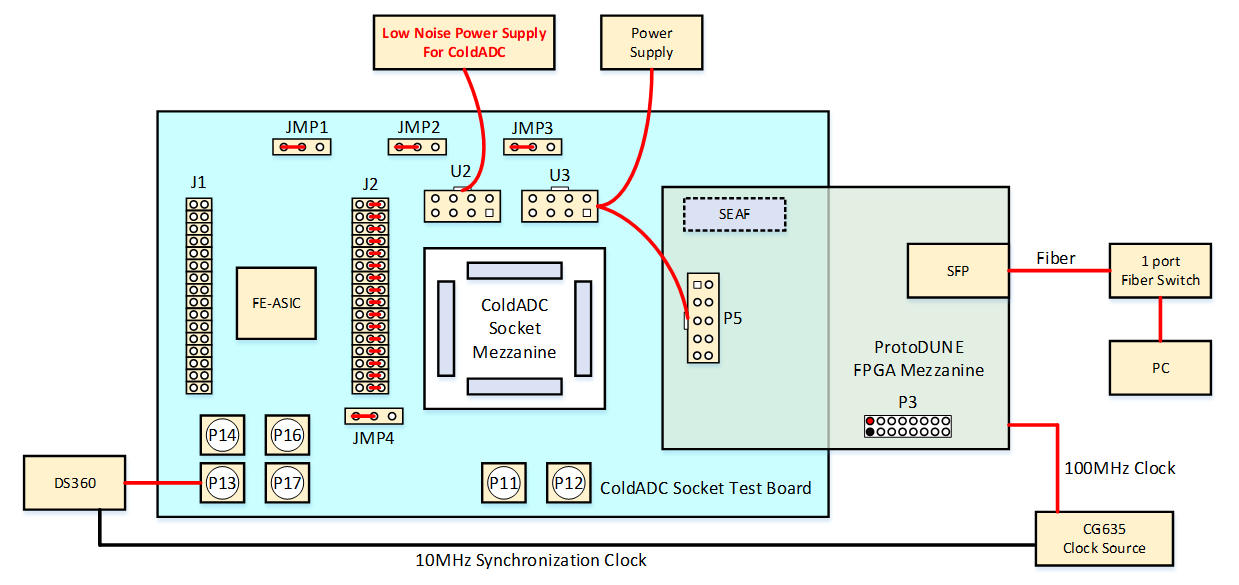
\includegraphics[width=0.8\linewidth]{figures/prodQC_blockdiagram.png}
  \caption{Block diagram of ColdADC Production Testing setup.}
  \label{fig:prodQC_blockdiagram}
\end{figure}
\begin{figure}[h!]
\centering
  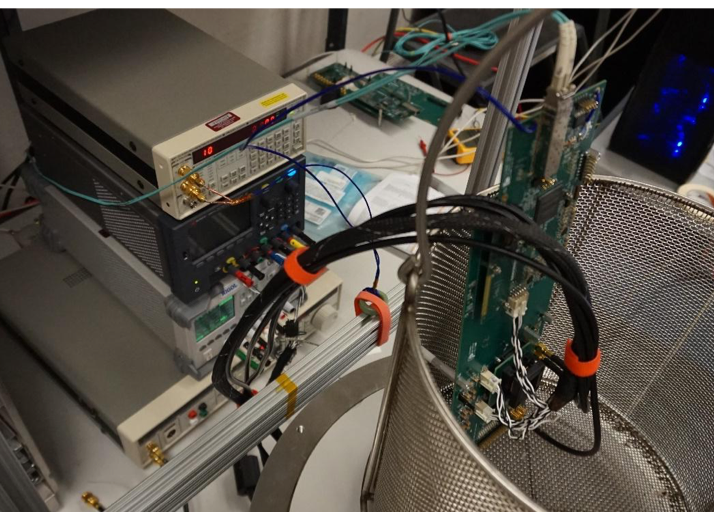
\includegraphics[width=0.7\linewidth]{figures/prod_warmsetup.png}
  \caption{ColdADC QC test setup at room temperature.}
  \label{fig:prod_warmsetup}
\end{figure}

The flowchart of the QC process is shown Figure~\ref{fig:qc_flowchart}.  The chart illustrates the sequence of steps for characterizing 
the functionality and performance of the chip. At every iteration, the measurements is done using BJT reference and then repeated 
again using the CMOS reference. 
%With a certain number of tested chips, it will be possible to highlight differences in performance between measurements taken 
%using one reference instead of the other. 
%The test flow includes input configuration, initialization checkout, static linearity (INL/DNL per channel), 
%Dynamic Behavior (ENOB/SFDR/SINAD per channel), DC noise per channel, and ADC core characterization. 
The list below describes the QC steps in more detail: 
\begin{enumerate}
\item Input configuration: ColdADC chip ID and test board ID are recorded, the path for data storage is specified. 
\item Initialization checkout: mainly to check ColdADC functionality. It includes power consumption with different 
configurations, power cycles, I2C/UART communication check, pattern and register check, reference sweeping check, 
synchronization and calibration check. Any chip failed in any procedure in this checkout is treated as a bad chip. 
\item  Static linearity: INL/DNL results are obtained with a sine wave input from the DS360 generator. Data and plots 
are generated with the sine wave code-density method. Performances at both 2 MS/s/ch and 500 kS/s/ch are measured.
\item Dynamic Behavior: ENOB/SFDR/SINAD is calculated from the FFT plot obtained by using coherent sampling. 
Performances at both 2 MS/s/ch and 500 kS/s/ch are measured. 
\item DC noise: Two DC points, 200mV and 900mV are chosen.
\item ADC core characterization (optional): DNL/INL, FFT, and DC noise. 
\end{enumerate}

The test procedure is largely automated using Python scripts. The only step that requires manual intervention is to replace the ASIC chips 
at the end of the measurement. When the test is completed, the Python script automatically generates a detailed report in pdf format. 
The report includes:
\begin{enumerate}
\item Summary: date and time, temperature, chip and board IDs, power consumption and characterization results (CMOS reference only, can be changed to BJT);
\item Initialization checkout: ADC power consumption with both BJT and CMOS references, sweep plots of reference voltages and currents;
\item Calibration weights: recorded weights listed with respect to internal ADC stages;
\item Noise study: RMS noise for each channel and comparison between all channels. Four pages in total: 200 mV and 900 mV baselines for both BJT and CMOS references;
\item Channels characterization: noise, linearity and dynamic studies, with both BJT and CMOS references for comparison. Each page collects results for one channel;
\item ADC test input: internal ADC characterization for two sampling rates, 4 MS/s and 16 MS/s.
\end{enumerate}
\begin{figure}[h!]
\centering
  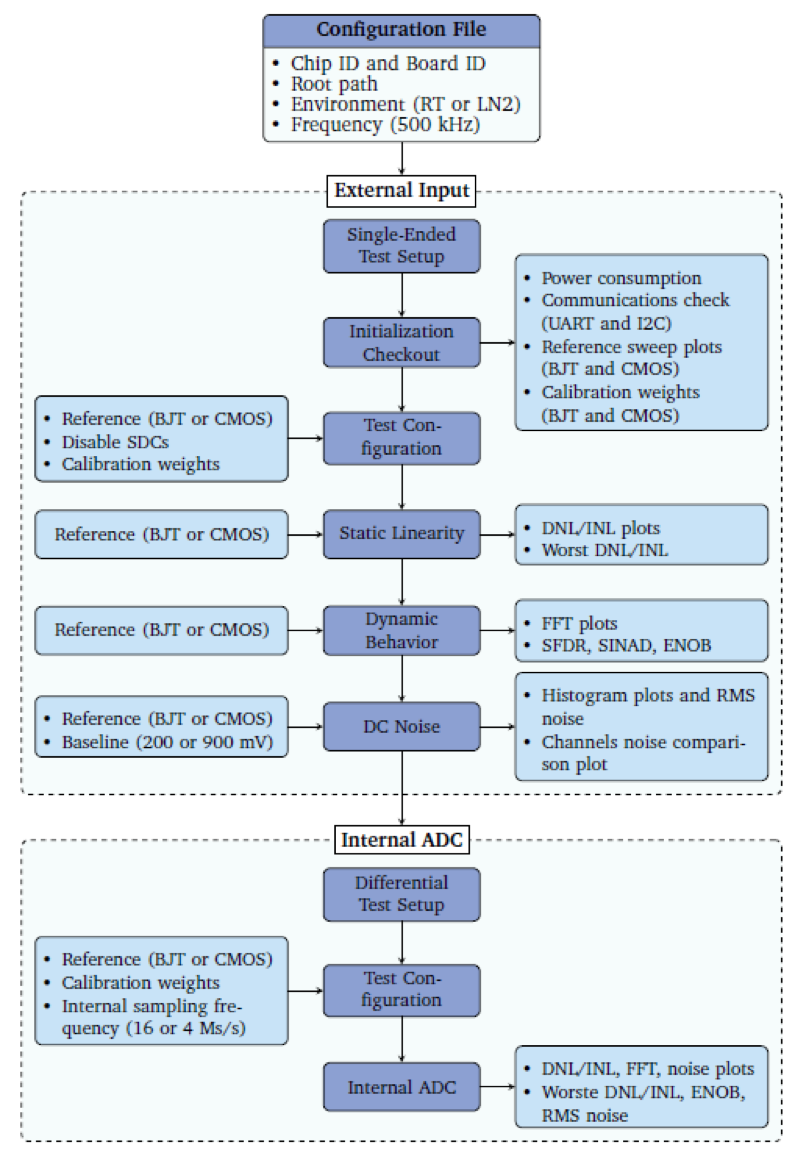
\includegraphics[width=0.8\linewidth]{figures/QC_flowchart.png}
  \caption{ColdADC QC Flowchart.}
  \label{fig:qc_flowchart}
\end{figure}

At the moment, the test data are stored in a local database at BNL. U. of Florida group is developing an online database for the ColdADC QC test that will be used for all future production tests.
%Ivan Furic research team from Florida University is going to develop an online database for the ColdADC QC test. BNL provides hardware, FPGA firmware, python scripts and necessary support to help them replicate the test procedure at BNL.  Florida University is responsible for QC test of 100 ColdADC chips in the coming two or three months. 

\subsection{Results}
\label{sec:6.2}
For the initial production QC test, a batch of 33 ColdADCs were tested. One of the chips (\#00096)  drew very high current (>1 A) when it 
was first powered and was excluded from further QC testing. It was found that the bad chip had a resistance of $<$ 5$\Omega$ between 
VDDA2P5 and VSSA2P5, while the nominal resistance should be about 12 k$\Omega$. The cause of the failure is not clear; may be due to 
manufacturing defect or handling issues. In additional to the 33 QC chips, 20 other chips were previously tested at BNL and passed 
functionality tests. Based on a sample of 53 chips (51 packaged and 2 bare dies), the functionality failure rate of ColdADC is less than 2\%.

\subsubsection{Power Consumption}
The power consumption of ColdADC strongly depends on the chip configuration. The power consumption with VDDA2P5/VDDD2P5=2.5V, 
VDDD1P2=2.1V, VDDIO=2.25V, SDC\&DB bypassed, CMOS reference, floating single-end input, and 2 MS/s sampling rate is summarized in in 
Figure~\ref{fig:qc_power}. For this configuration, the average power consumption of ColdADC is about 413 mW at room and 450 mW at LN$_2$ temperature.
\begin{figure}[h!]
\centering
  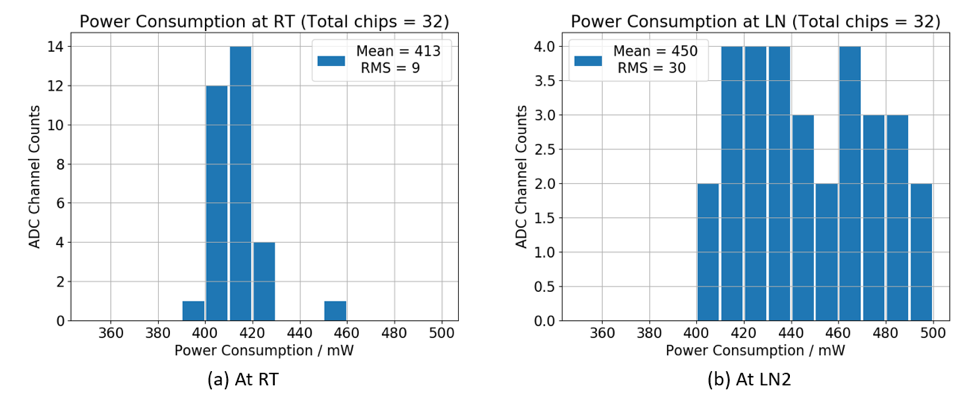
\includegraphics[width=0.85\linewidth]{figures/qc_power.png}
  \caption{Power consumption distribution.}
  \label{fig:qc_power}
\end{figure}

\subsubsection{Linearity Results with 2 Ms/s/channel Sampling Rate}
The results of the linearity and noise measurements at the nominal 2 Ms/s/channel sampling rate for the 33 chips are shown in 
Figures~\ref{fig:qc_lin2Mwarm} (RT) and Figure~\ref{fig:qc_lin2Mcold} (LN$_2$). 
%The degradation is allowed because it is consistent to all chips, and additional test with 500 kS/s per 
%channel is also performed to confirm the degradation is caused by SHA/MUX crosstalk issue.  
%The ColdADC internally is 16-bit. The DUNE experiment requires 12-bit ADC is required by 
%DUNE experiment, ColdADC is truncated down to 12-bit by cut-off the lowest 4 bits. Meanwhile, in order to get ENOB, the coherency 
%frequency of sine wave is calculated for 12-bit ADC followed the equation of IEEE standard. 
Overall, the ColdADC performance is reasonably good, average of the worst DNL is 0.76 LSB, average of the worst INL is 2.6 LSB, 
average of ENOB is 10.0 bit and average of DC noise at 900mV is 0.68vLSB. In addition, the spread of these 4 key parameters 
among channels (or chips) is small.
Cryogenic test is performed as well with the same configuration,  Figure 7 shows the statistical result. 
By comparing Figure 6 and Figure 7, the linearity  performance of DNL, INL and ENOB do not show significant temperature dependence
 but the DC noise at LN$_2$ is smaller than at RT due to the suppression of thermal noise at cryogenic temperature.  
The linearity results shown here are slightly worse than the ones shown in Section~\ref{sec:4} due to the known SHA/MUX crosstalk issue.
For the QC tests, all 16 input channels are simultaneously connected to the signal source.
Another caveat for the QC results is that the calibration of the ADC pipeline stages are not done to shorten the testing cycle time.

\begin{figure}[h!]
\centering
  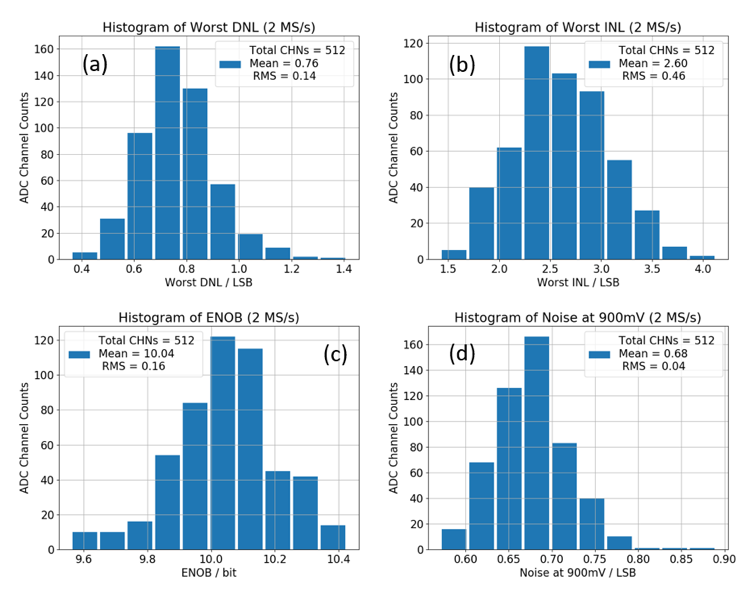
\includegraphics[width=0.85\linewidth]{figures/qc_lin2Mwarm.png}
  \caption{ColdADC QC Results at RT with 2 MS/s per channel sampling rate. ADC output is trucated to 12-bit.}
  \label{fig:qc_lin2Mwarm}
\end{figure}
\begin{figure}[h!]
\centering
  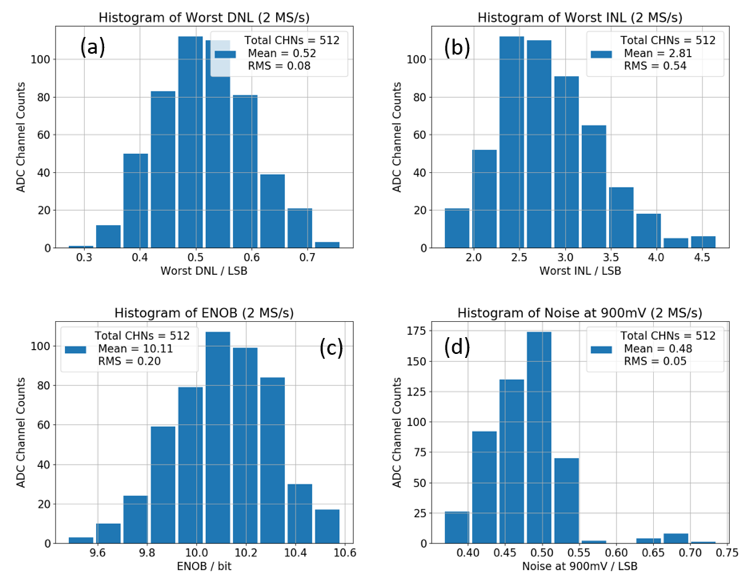
\includegraphics[width=0.85\linewidth]{figures/qc_lin2Mcold.png}
  \caption{ColdADC QC Results at LN$_2$ temperature with 2 MS/s per channel sampling rate. ADC output is trucated to 12-bit.}
  \label{fig:qc_lin2Mcold}
\end{figure}



\subsubsection{Linearity Results with 0.5 Ms/s/channel Sampling Rate}
The SHA/MUX crosstalk issue mentioned in the earlier section is expected to be fixed in the next revision of the ColdADC.
For now we can estimate the optimized performance without the crosstalk issue by repeating the QC measurements with a slower 
sampling rate and still pulse all 16 channels simultaneously.
Results at a sampling rate of 0.5 Ms/s per channel are shown in Figures~\ref{fig:qc_lin500Kwarm} (RT) and Figure~\ref{fig:qc_lin500Kcold} (LN$_2$). 
%To predict the possible optimized performance of revision (if the SHA/MUX crosstalk issue is fixed), the QC test for each chip is conducted with ColdADC working at 500 kS/s per channel as well, as shown in Figure 8 is the result at room temperature and Figure 9 is the result at cryogenic temperature. 
Compared to the result of 2MS/s per channel, the linearity is significantly better. Average of the worst INL/DNL is less than 1 LSB.
Average of ENOB is nearly 11 bits at LN$_2$.  DC noise at room temperature is improved but no significant difference is observed at LN$_2$.
%however, the DC noise is lower enough. 
\begin{figure}[h!]
\centering
  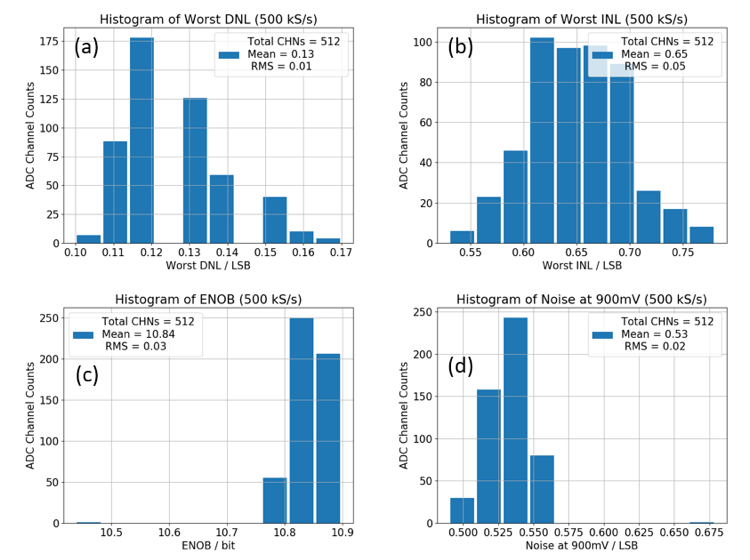
\includegraphics[width=0.85\linewidth]{figures/qc_lin500Kwarm.png}
  \caption{ColdADC QC Results at RT with 0.5 MS/s per channel sampling rate. ADC output is trucated to 12-bit.}
  \label{fig:qc_lin500Kwarm}
\end{figure}
\begin{figure}[h!]
\centering
  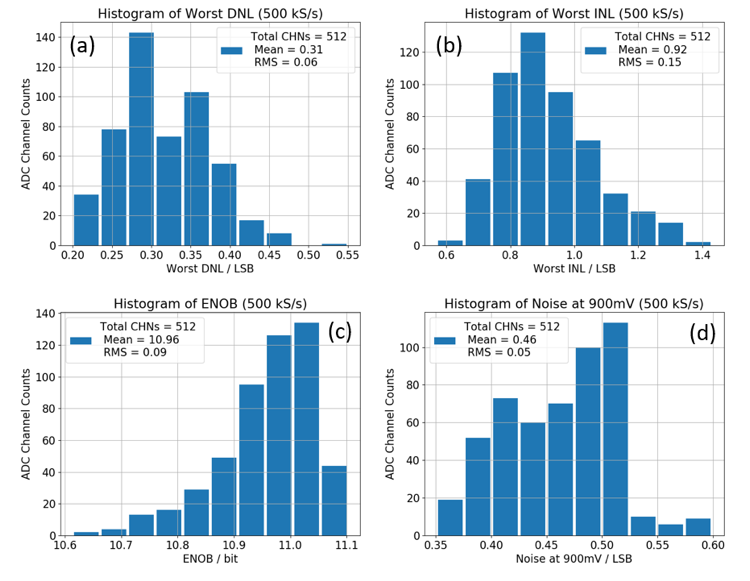
\includegraphics[width=0.85\linewidth]{figures/qc_lin500Kcold.png}
  \caption{ColdADC QC Results at LN$_2$ temperature with 0.5 MS/s per channel sampling rate. ADC output is trucated to 12-bit.}
  \label{fig:qc_lin500Kcold}
\end{figure}
